\documentclass[a0paper]{sciposter}
\RequirePackage[utf8,utf8x]{inputenc}
\usepackage{url}
\usepackage{multicol}
\usepackage{graphicx}
\usepackage{color}
\usepackage{subfig}
\usepackage[dvips,dvipdfm,top=4cm,bottom=10cm,left=4cm,right=8cm]{geometry}

% usar para termos estrangeiros
\newcommand{\eng}[1]{\textit{#1}}

\newcommand{\rameau}[1]{\textit{Rameau}}

\renewcommand{\papertype}{a0paper}
\renewcommand{\fontpointsize}{25pt}

% \setlength{\paperwidth}{85cm}
% \setlength{\paperheight}{127cm}
% \renewcommand{\setpspagesize}{
%   \ifthenelse{\equal{\orientation}{portrait}}{
%     \special{papersize=85cm,127cm}
%     }{\special{papersize=127cm,85cm}
%     }
%   }

\definecolor{SectionCol}{rgb}{1,1,1}
\definecolor{BoxCol}{rgb}{.230,.230,.76}

\def\abovestrut#1{\rule[0in]{0in}{#1}\ignorespaces}
\def\belowstrut#1{\rule[-#1]{0in}{#1}\ignorespaces}

\def\abovespace{\abovestrut{0.20in}}
\def\aroundspace{\abovestrut{0.20in}\belowstrut{0.10in}}
\def\belowspace{\belowstrut{0.10in}}

\title{Functional Harmonic Analysis and Computational Musicology in
  Rameau}

\author{Alexandre Tachard Passos, Marcos Sampaio, Pedro Kröger,
  Givaldo de Cidra}

\institute{Genos---Computer Music Research Group \\
Federal University of Bahia (UFBA). Salvador, Brazil}

\email{pedro.kroger@gmail.com}

% The following commands can be used to alter the default logo settings
% \leftlogo[.7]{figs/ufba-logo}{  % defines logo to left of title (with scale factor)
% \rightlogo[1.1]{figs/capes-logo}  % same but on right

\begin{document}

\bibliographystyle{plain}

\conference{\Large \textbf{XII SBCM --- 2009
    \hfill \textsf{GENOS Research Group}}}

\maketitle

\begin{multicols}{3}

\section{Introduction}
\label{sec:introduction}

In the past few years we have been developing Rameau, an open-source
system for automatic harmonic analysis and computational musicology
\cite{kroger08:rameau}. With Rameau one can process Lilypond files to
generate typeset harmonically analysed scores, identify non-chordal
sonorities and label chords, perform some basic musicological tasks
(such as cadence and voice crossing detection). Rameau is written in
Common Lisp and its source code can be found in
\url{http://genos.mus.br/rameau/}, together with the data set of Bach
chorales from the Riemenschneider \cite{bach41:371} edition we use to
benchmark and test the system. In this paper we present Rameau's
infrastructure for computational musicology and Rameau's
implementation of a functional harmonic analysis framework.

The organization of this paper is as follows; section \ref{sec:system}
gives an overview of how Rameau works, section \ref{sec:comp-music}
presents the main musicological features implemented in the
system. Section \ref{sec:problem} describes the functional harmonic
analysis structure of Rameau. Section \ref{sec:algorithms} describes
superficially each algorithm currently implemented in Rameau. Section
\ref{sec:concl-future-work} contains some concluding remarks and
directions for future work.

\section{Overview of Rameau}
\label{sec:system}

There are two ways of accessing Rameau: a comprehensive command-line
interface and a simple web server to perform functional harmonic
analysis. When starting the command-line interface the user can choose
which Lilypond files are to be processed and what to do with
them. The possible operations are called \textit{commands}, and some
of the available commands are:
\begin{itemize}
\item \textbf{help}: provides help and describes the other commands
  individually;
\item \textbf{octaves}: identifies parallel octaves in the specified files;
\item \textbf{crossings}: detects voice crossings in the specified
  bach chorales;
\item \textbf{cadences}: detects the cadences in the specified files;
\item \textbf{analysis}: identifies non-chordal sonorities and name
  the chords in the specified files, with many different algorithms;
\item \textbf{functional}: performs functional harmomnic analysis of
  the given files;
\item \textbf{document}: generates html documentation for the Rameau
  source code.
\end{itemize}
There are altogether 26 different commands, and a new useful command
can be implemented in five lines of common lisp code.

Musicological commands can output their data in many formats, such as
a typeset score of the interesting section of the song, a list of
interesting matches, a histogram of interesting matches and a cloud
plot of the extracted data. The harmonic analysis commands
(\textbf{functional} and \textbf{analysis}) can generate tabular
results and annotated typeset scores.

\section{Computational musicology}
\label{sec:comp-music}

The commands \textbf{octaves} and \textbf{fifths} show how many
consecutive octaves and fifths are in a piece and where they are. We
found that all consecutive octaves in Bach Chorales are in the form
unison--octave or octave--unison, but no consecutive octaves in all
Chorales are parallel, although a few fifths are (in chorales 4, 46,
71, and 266). More information can be found in
\cite{kroger08:musicologia}.


The command \textbf{chords} lists the frequency of each type of chord
in a set of chorales. The command \textbf{crossings} finds passages where
are voice crossings. We found that in 57\% of the Bach chorales there
is some kind of voice crossing, although most of the crossings happen
in a short period of time (no more than two beats). There are a few
interesting cases. For instance, the alto is the lowest voice for a
brief period of time in chorale \#35 and there is a crossing of the
soprano and alto and tenor and bass at the same time in chorale \#
290.

There are also commands to find the vocal range used in a composition
(\textbf{kostka-amb}), to find melodic jumps in a voice
(\textbf{jumps}), to collect statistics on seventh notes' resolution
(\textbf{resolve-seventh}), to collect data on how many chord
progressions found in the chorales are strong, weak, superstrong and
neutral, according to Schoenberg's theory of harmony
\cite{schoenberg83:theory} (\textbf{schoenberg}), to detect the final
cadences in the analyzed pieces (\textbf{cadences}), and to count the
notes found in major and minor modes (\textbf{count-major-notes} and
\textbf{count-minor-notes}).

\section{The functional harmonic analysis structure of Rameau}
\label{sec:problem}

Roman numeral functional analysis consists, roughly, of two
activities: key finding---determining what is the tonal center of the
piece and its parts---and roman numeral function
detection---determining the tonal function of each segment of the
piece. In Rameau we chose to merge these two conceptual concerns into one,
and the internal representation chosen reflects that, by stating that
the analysis of a song is a list of the analyses of every distinct
sonority in the song, and the analysis for each sonority is a local
key, mode, and tonal function.

One of the goals of the Rameau project to understand and compare
previously published and new techniques for automatic harmonic
analysis. To properly compare harmonic analysis algorithms we have a
corpus of 371 Bach chorales from the Riemenschneider edition
\cite{bach41:371}, 20 of them annotated by experts with an acceptable
harmonic analysis. Rameau includes facilities to train machine
learning algorithms on these analyzed chorales (commands named
\textbf{algorithms} and \textbf{funalg} for chord-labeling and
functional analysis algorithms, respectively) and a bayesian framework
for estimating the correctness of the expert annotations and using
this estimate to derive confidence intervals for the accuracies of the
algorithms (command named \textbf{information-theory}). The analysis
results are automatically typeset with the aid of the Lilypond music
typesetting program \cite{nienhuys.ea08:lilypond}.

\section{Functional harmonic analysis algorithms}
\label{sec:algorithms}

Using the infrastructure described in section \ref{sec:problem}
Rameau currently has implementations of four different roman numeral
functional analysis; a hidden Markov model, a k-nearest neighbors
classifier, a neural network-based harmonic analyzer similar to the
one described by Tsui \cite{tsui02:harmonic}, and a trivial extension
of Pardo \& Birmingham's chord labeling algorithm
\cite{pardo.ea99:automated}.

\subsection{Hidden Markov Model}
\label{sec:hidden-markov-model}

A hidden Markov model is any probabilistic function of a Markov
chain. Using a hidden Markov model to perform roman numeral function
analysis consists of modeling the notes in a tonal piece as a
probabilistic function of the underlying harmonies, and finding these
harmonies, given the notes, using traditional hidden Markov model
algorithms. Our approach closely follows that of Raphael and Stoddard
\cite{raphael.ea03:harmonic}, and the differences are noted in
\cite{passos08:modelos}.


\subsection{K-Nearest Neighbors}
\label{sec:knn}

A tool used in machine learning for many non-trivial tasks is the
k-nearest neighbors classifier \cite{mitchell97:machine}. It works by
first representing the instances to be classified in some metric
space. Then, to classify an instance $x$, the knn algorithm chooses,
from the training data set, the set $s$ of the $k$ closest examples to
$x$ and outputs the most common class in $s$. The spatial
representation we chose for Rameau is a pitch frequency array $a$, in
which, if $f*n$ on the $n$ pitches in a given sonority are encoded as
having number $p$, then $a[p] = f$. When considering surrounding
context, we concatenate these arrays and, to avoid adding too much
noise in the distance function we weight them down in proportion to
the square of the distance between the contextual sonority and the
sonority being analyzed. More details can be found in
\cite{passos08:modelos}.

\subsection{Pardo \& Birmingham's}
\label{sec:pardo--birminghams}

Pardo \& Birmingham \cite{pardo.ea99:automated} describes an algorithm
for chord labeling that has some predefined chord templates and
chooses among them the one that most closely matches the notes
sounding in a given sonority. To extend the original algorithm to
perform roman numeral functional analysis we simply created the key
for the whole piece using the root and mode of the first chord found,
and thus computed the roman numeral function for all other chords as
if they were in that key. While simplistic, this approach performs
almost competitively with the hidden Markov model.

\end{multicols}

\begin{center}
\begin{multicols}{2}

\begin{figure}
  \centering
  \includegraphics[scale=1]{rameau-web}
  \caption{Rameau's web interface}
  \label{fig:rameau-web}
\end{figure}

\begin{figure}
  \centering
  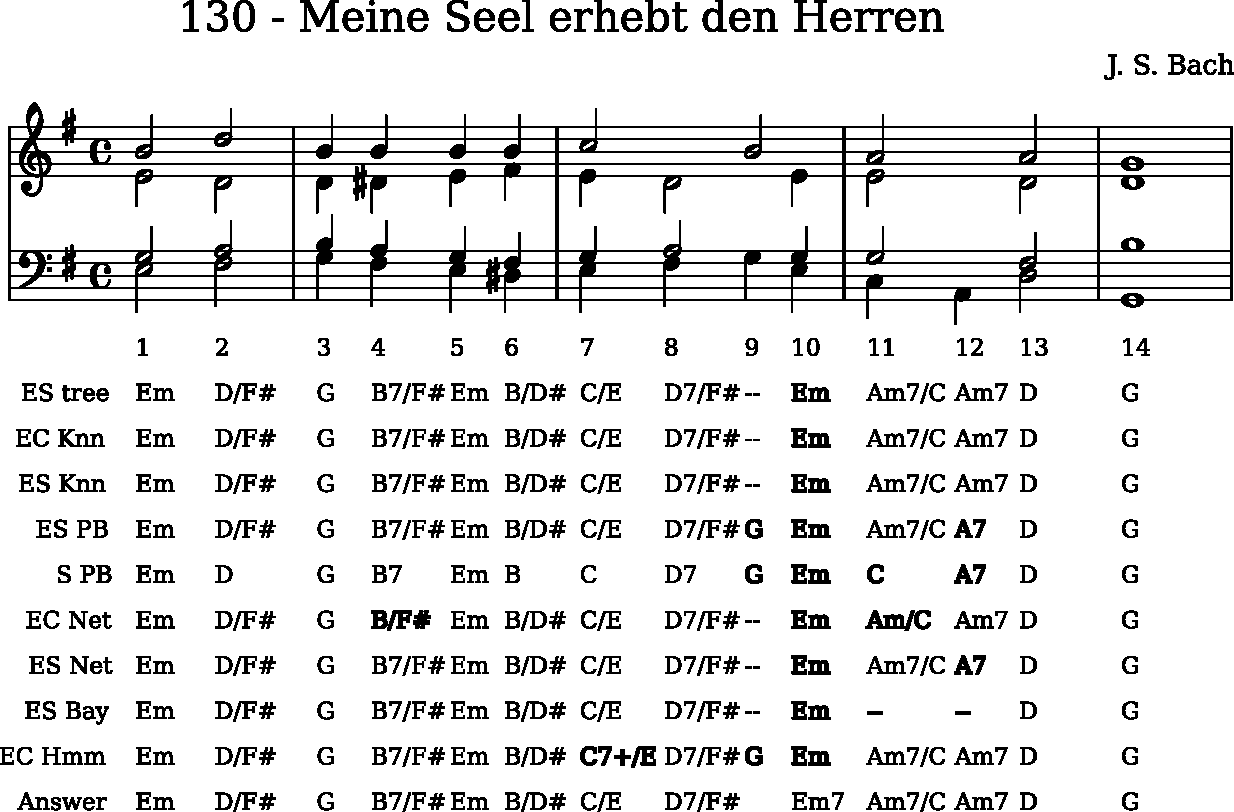
\includegraphics[scale=1]{analysis-130}
  \caption{Chord name analysis}
  \label{fig:chord-name-analysis}
\end{figure}
\begin{figure}
  \centering
  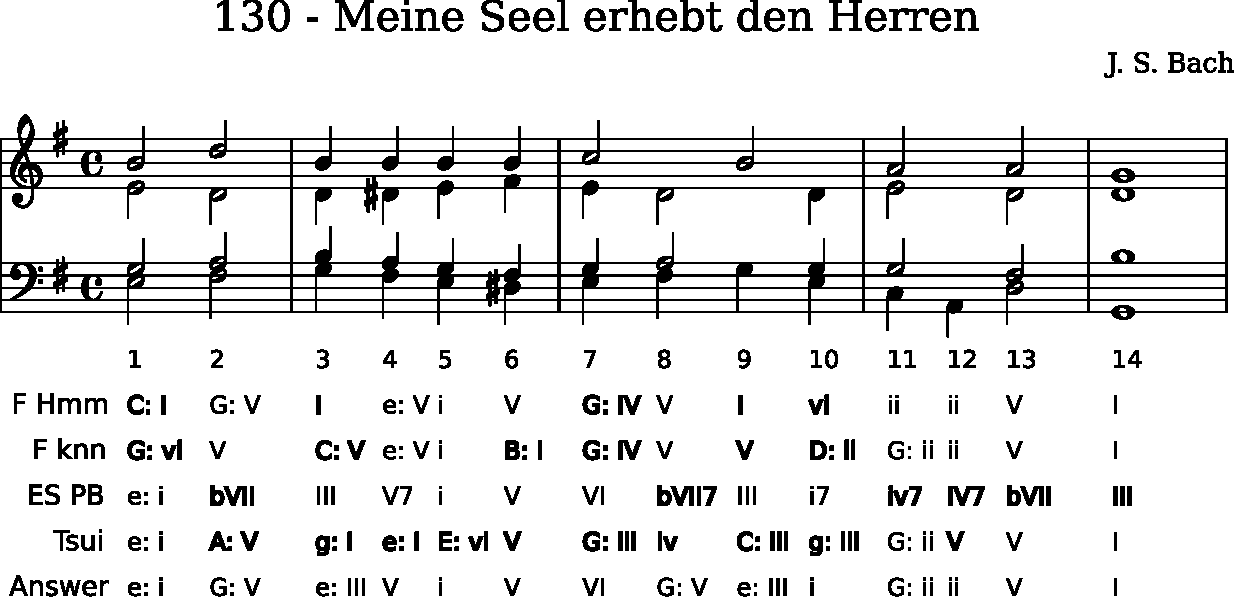
\includegraphics[scale=1]{analysis-functional-130}  
  \caption{Roman numeral analysis}
  \label{fig:roman-analysis}
\end{figure}

\begin{figure}[!h]
  \centering
  \subfigure[Chorale \#244]{
    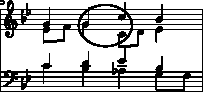
\includegraphics[scale=2]{244-oitava}
    \label{fig:244-oitava}
  }
  \qquad
  \subfigure[Chorale \#279]{
    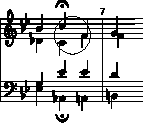
\includegraphics[scale=2]{279-oitava}
    \label{fig:279-oitava}
  }
  \qquad
  \subfigure[Chorale \#329]{
    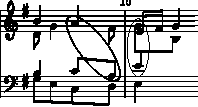
\includegraphics[scale=2]{329-oitava}
    \label{fig:329-oitava}
  }
  \caption{Consecutive octaves and unisons}
  \label{fig:oitavas-e-unissonos}
\end{figure}

\begin{table}[t]
  \centering
\begin{tabular}{l|l} \hline
 Chord type & Frequency (\%) \\ \hline
 C/F\#                & 4.2 \\
 C/D\#                & 4.2\\
 C/E                 & 4.2\\
 Cm7/C               & 4.2\\
 Cm7                 & 4.2\\
 C/B                 & 4.2\\
 Cm/C                & 4.2\\
 Cm/B                & 4.2\\
 C7                  & 4.2\\
 C7/F\#               & 8.3\\
 --                  & 8.3\\
 Cm                  &16.7\\
 C                   &29.2 \\ \hline
\end{tabular}
\caption{Chord types in in chorale \# 130}
\label{tab:ctc130}
\end{table}

\begin{figure}[!h]
  \centering
  \subfigure[Chorale \#35]{
    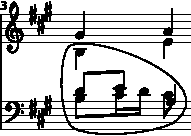
\includegraphics[scale=2]{035-16-20-cruzamento}
    \label{fig:035-cruzamento}
  }
  \subfigure[Chorale \#290]{
    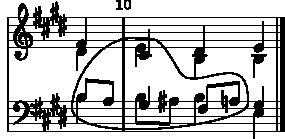
\includegraphics[scale=2]{290-66-74-cruzamento}
    \label{fig:290-66-74-cruzamento}
  }
  \caption{Voice crossing}
  \label{fig:coral-003}
\end{figure}

\begin{figure}
  \centering
  \includegraphics[scale=1]{cadences}
  \caption{Final cadences in Bach Chorales}
  \label{fig:cadences}
\end{figure}

\begin{figure}[t]
  \centering
  \includegraphics[scale=1.5,trim=0cm 5cm 0cm 2.5cm]{amostra-markov}
  \caption{A sample from the hidden Markov model}
  \label{fig:amostra}
\end{figure}

\begin{algorithm}[t]
%   \SetLine
%   \KwIn{$x$, an instance to be classified}
%   $nearest = nil$\;
%   $distance = \infty$\;
%   \For{each example $e$}{
%     \If{$d(e,x) < distance$}{
%       $nearest = e$\;
%       $distance = d(e,x)$\;
%     }
%   }
%   \KwRet{$class(nearest)$}\;
  \caption{A nearest neighbor classifier (a knn for $k=1$).}
  \label{alg:knn}
\end{algorithm}

\begin{table}[h]
  \centering
  \begin{small}
    \begin{sc}
      \begin{tabular}[t]{ll} \hline
        Chord type & Notes (counting from c) \\ \hline
        Major triad & c e g \\
        Major-minor chord &  c e g b$\flat$ \\
        Minor triad & c e$\flat$ g \\
        Minor-minor chord & c $e\flat$ g b$\flat$ \\
        Fully diminished chord & c e$\flat$ g$\flat$ b$\flat\flat$ \\
        Half-diminished chord & c e$\flat$ g$\flat$ b$\flat$ \\
        Diminished triad & c e$\flat$ g$\flat$ \\
        Major-major chord & c e g b \\
        Augmented triad & c e g$\sharp$ \\
        German sixth  & c e g a$\sharp$ \\
        Italian sixth & c e a$\sharp$ \\
        French sixth & c e f$\sharp$ a$\sharp$ \\ \hline
      \end{tabular}
    \end{sc}
  \end{small}
  \caption{Templates for the Pardo \& Birmingham algorithm.}
  \label{tab:templates-pardo}
\end{table}


\end{multicols}
\end{center}


\begin{multicols}{3}

\section{Conclusions and future work}
\label{sec:concl-future-work}

In this paper we presented the current status of Rameau, a framework
for automatic harmonic analysis and computational musicology. The
framework is mature, and has implementations of many useful
musicological functions. The architecture is still too tied to 4-voice
part writing, command-line operation, and the Lilypond format, but we
are working to correct this in future releases.

While still preliminary, the current implementation of functional
harmonic analysis in Rameau is promising, and already produces useful
results. Rameau has implementations of a hidden Markov model, a
K-nearest neighbors, Pardo \& Birmingham's, and neural networks
functional harmonic analysis algorithms. Rameau is open source,
written in Common Lisp and its source code (together with our data
sets and instructions on how to compile, install and run it) is
available at \url{http://genos.mus.br/rameau/}.

\renewcommand{\refname}{References}

\bibliography{strings-short,bibliography,computer-music,ismir,writing-style,harmonic-analysis,music-analysis,computational-musicology,melodic-contour,music-harmony-and-theory,programs,music-scores,genos}

\end{multicols}

\end{document}